%!TEX root = ../my_thesis.tex
\chapter{Implémentation logicielle des algorithmes de décodage à Liste} % (fold)

% Intro chapitre

\vspace*{\fill}
\minitocTITI
\vspace*{\fill}
\newpage


\section{Introduction}

\begin{figure}[t]
  \centering
  \subfloat[Stations de bases traditionnelle]{
  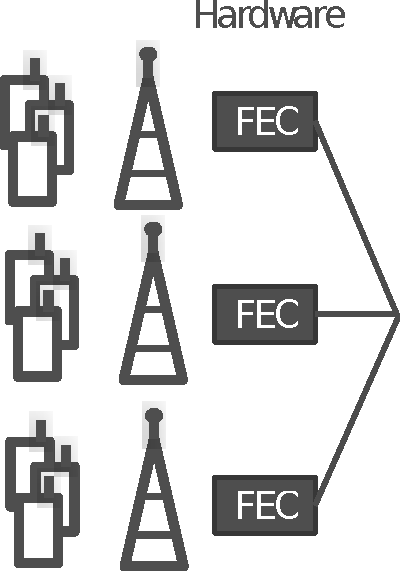
\includegraphics[scale=0.5]{main/ch2_fig/bs}
  \label{fig:bs}
  }
  \quad\quad
  \subfloat[Séparation BBU / RF]{
  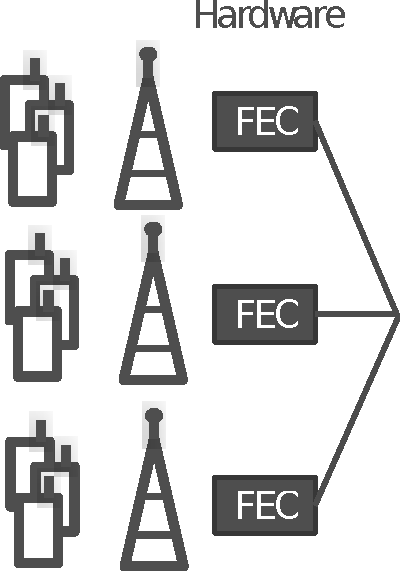
\includegraphics[scale=0.5]{main/ch2_fig/bs}
  \label{fig:bbu}
  }
  \quad\quad
  \subfloat[Cloud-RAN]{
  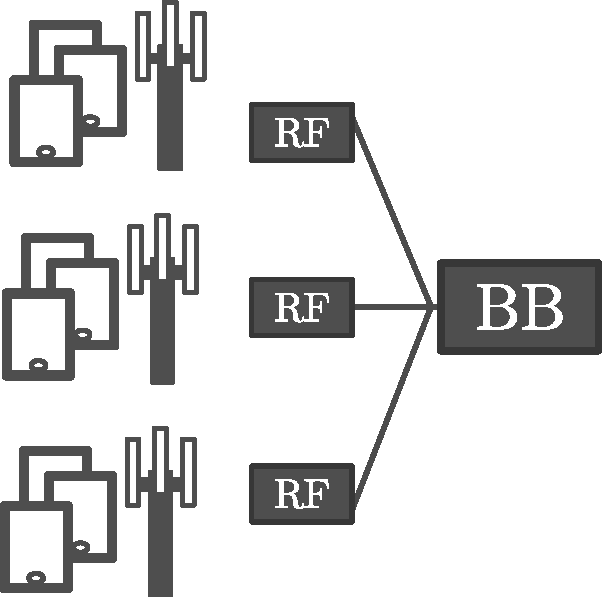
\includegraphics[scale=0.5]{main/ch2_fig/c-ran}
  \label{fig:c-ran}
  }
  \caption{\'Evolution de l'architecture des stations de base}
  \label{fig:bs_evo}
\end{figure}

La virtualisation des réseaux radio mobiles est considérée par les acteurs industriels \cite{ericsson_cloud_2015,huawei_5g:_2013,checko_cloud_2015} comme académiques \cite{wubben_benefits_2014,rost_cloud_2014} comme une fonctionnalité prometteuse. Elle est illustrée en Figure~\ref{fig:bs_evo}. Dans les premières génération, 1G et 2G illustrées en Figure \ref{fig:bs}, toutes les étapes de traitement du signal sont réalisées dans la station de base, à proximité de l'antenne, comme montré en Figure~\ref{fig:bs}. Une première évolution introduite dans les réseaux 3G est la séparation des traitements en bande de base (BBU : Base Band Unit) d'un coté et des traitements fréquence radio (RF : radio frequency) de l'autre. Comme représenté en Figure~\ref{fig:bbu} tandis que la BBU, distante de l'antenne, s'occupe du traitement en bande de base, dont le codage canal, la cellule RF a uniquement pour rôle la conversion du signal en signal RF. L'avantage de cette évolution est de pouvoir placer les stations BBU plus proches des centres urbains pour faciliter la maintenance.

L'étape suivante est nommée Cloud-RAN (Cloud Radio Access Network). Un groupe de BBUs est alors partagé entre plusieurs antennes et des optimisations entre BBUs peuvent être envisagées. Ces optimisations doivent permettre i) une meilleure adaptabilité aux traffics non uniformes, ii) des économie d'énergie, iii) des augmentations de débits et des réductions de la latence et enfin iv) de meilleures évolutivités et maintenabilité. Pour cela, ces BBUs doivent être virtualisées. Il ne doit plus y avoir un support matériel unique pour chaque BBU, mais au contraire, les calculs doivent être distribué sur le Cloud. Pour que cela soit réalisable, il est nécessaires que tous les algorithmes exécutés par les BBUs soient implémentés logiciellement. Or le décodage canal est une des tâches les plus intensives en calcul de l'ensemble des traitements en bande de base \cite{rodriguez_towards_2017,nikaein_processing_2015}. Ainsi, des implémentations efficaces et flexibles de codes correcteurs d'erreurs, comme celles présentées dans ce chapitre, sont nécessaires.

Ce chapitre est divisé comme suit. Tout d'abord, l'état de l'art des implémentations logicielles des algorithmes SC et SCL sur des processeurs à usage général est présenté dans la Section~\ref{sec:art_scl}. Les principales techniques permettant d'atteindre de hauts débits et de faibles latences sont détaillées. Un effort particulier a été réalisé afin de rendre les implémentations proposées génériques et flexibles. Dans un souci de clarté, les concepts de généricité et de flexibilité sont définis précisément et leurs implications sont détaillées dans la Section~\ref{sec:gen_scl}. Pour atteindre des débits et des latences compétitifs, des optimisations d'implémentations ont été proposées et sont décrites en Section \ref{sec:opti_scl}. Enfin, en Section~\ref{sec:exp_scl} les implémentations proposées sont comparées entre elles et avec l'état de l'art.

\section{\'Etat de l'art des implémentations logicielles d'algorithmes de décodage de codes polaires}
\label{sec:art_scl}

\subsection{Vectorisation}
Les processeurs à usage général (GPPs : General Purpose Processors) modernes sont de manière générale équipés d'unités de calcul vectoriel SIMD (Single Instruction Mutiple Data). Les architectures de processeurs x64 définissent par exemple des jeux d'instructions SIMD allant jusqu'à des tailles de 256 bits. Ces instruction incluent des opérations de chargement, sauvegarde et de mélange afin d'accéder aux données en mémoire et de les déplacer à des endroits voulus dans le registre, ainsi que des opérations de calcul, comme les additions, soustraction, multiplication.

Réduire le temps de décodage des algorithmes de décodage de codes polaires est une technique classique utilisée dans de nombreuses implémentations pour l'algorithme SC \cite{giard_fast_2014,giard_low-latency_2016,sarkis_fast_2014,sarkis_autogenerating_2014,giard_low-latency_2016,gal_software_2014,cassagne_efficient_2015,cassagne_energy_2016} comme pour l'algorithme SCL \cite{sarkis_increasing_2014,sarkis_fast_2016,shen_low-latency_2016}. Dans nos travaux est utilisée une librairie générique et portable implémentant les fonctions élémentaires des codes polaires \cite{cassagne_efficient_2015}. Elle est basée elle-même sur la librairie MIPP \cite{cassagne2018mipp} qui est une encapsulation des instructions SIMD dont la description logicielle est écrite dans le langage C++.

  \lstset{linewidth=0.7\textwidth, xleftmargin=0.025\textwidth, xrightmargin=0.05\textwidth}

  \begin{figure}[t]
  \begin{lstlisting}[language=C++, numbers=left, numbersep=0.3em, tabsize=2, basicstyle=\footnotesize\ttfamily]
class API_polar
{
  template <typename R>
  mipp::Reg<R> f_simd(const mipp::Reg<R> &la,
                      const mipp::Reg<R> &lb)
  {
    auto abs_la  = mipp::abs(la);
    auto abs_lb  = mipp::abs(lb);
    auto abs_min = mipp::min(abs_la, abs_lb);
    auto sign    = mipp::sign(la, lb);
    auto lc      = mipp::neg(abs_min, sign);

    return lc;
  }

  template <typename B, typename R>
  mipp::Reg<R> g_simd(const mipp::Reg<R> &la,
                      const mipp::Reg<R> &lb,
                      const mipp::Reg<B> &sa)
  {
    auto neg_la = mipp::neg(la, sa);
    auto lc     = neg_la + lb;

    return lc;
  }

  template <typename B>
  mipp::Reg<B> h_simd(const mipp::Reg<B>& sa,
                      const mipp::Reg<B>& sb)
  {
    return sa ^ sb;
  }
};
  \end{lstlisting}
  \caption{Implémentation des fonctions $f$, $g$ et $h$ utilisant la librairie MIPP.}
  \label{fig:mipp}
  \end{figure}
L'utilisation de cette librairie présente plusieurs avantages. Premièrement le code source apparaît clair, lisible et compact, contrairement à ce qui serait obtenu en utilisant le langage assembleur. Un extrait du code est donné en Figure~\ref{fig:mipp}. Deuxièmement, ce code source est portable. En effet, le code ainsi obtenu est compatibles avec différentes cibles matérielles (Intel x86, Xeon KNL et ARM) et il est possible d'utiliser différents jeux d'instructions (SSE, AVX, AVX-512, NEON). Troisièmement, plusieurs formats de représentation des données réelles sont utilisable : virgule flottante sur des mots de 32 bits, virgule fixe sur des mots de 8 ou 16 bits. Cette versatilité est obtenue sans perte de performance comme démontré dans \cite{cassagne2018mipp}.

Dans le contexte du décodage de codes polaires comme évoqué en Section \ref{subsubsec:parallel}, il existe deux stratégies principales afin d'utiliser le parallélisme SIMD. Les éléments d'un registre sont utilisés soit pour décoder de multiples trames en parallèle (\textit{inter-trame}), soit pour accélérer le décodage de chaque trame prise individuellement (\textit{intra-trame}). Dans les travaux présentés ici, seuls la stratégie \textit{intra-trame} est utilisée. L'avantage de cette technique est une latence inférieure. Le principe est d'utiliser le parallélisme disponible grâce aux fonctions $f$, $g$ et $h$ qui peuvent être effectués simultanément sur les \noeuds de grande taille, donc en haut de l'arbre, comme précisé toujours en Section \ref{subsubsec:parallel}. Il est également possible d'utiliser des instructions SIMD pour réaliser les opérations sur les feuilles. En effet, que ce soit dans les feuilles de type \texttt{R1}, \texttt{REP} ou \texttt{SPC}, il est nécessaire d'effectuer des opérations de seuillage sur un nombre de LLRs correspondant à la taille du \noeud. Ce seuillage est effectué parallèlement sur chacun de ces LLRs grâce à des instructions SIMD.

Toutefois, le parallélisme n'est utilisable que dans la partie supérieure de l'arbre, lorsque les \noeuds sont de tailles supérieure au parallélisme des unités SIMD. Dans le bas de l'arbre, près des feuilles, la librairie polaire \cite{cassagne_efficient_2015} utilise automatiquement les versions séquentielles des implémentations des fonctions élémentaires. Dans le cas de l'algorithme CASCL sur un code polaire de taille (2048, 1723) permet une augmentation du débit d'environ 20\%.


\subsection{Déroulage}
\label{subsec:unroll}
Une deuxième technique utilisée dans les travaux récents est le déroulage du code source \cite{sarkis_autogenerating_2014,giard_fast_2014,cassagne_efficient_2015,cassagne_energy_2016}. Il découle de l'observation faite sur les décodeurs de l'algorithme SC qu'un temps non négligeable est passé lors de différents tests au cours du parcours de l'arbre. Or il est possible d'éviter ces tests en générant un code source déroulé avant la compilation. Une illustration de ce déroulage est donnée en Figure~\ref{fig:unrolling}. D'un coté, dans le code non déroulé en Figure \ref{fig:alg_rolled}, des appels récursifs de la fonction \textit{DecodeNode} sont réalisés, qui peuvent être coûteux. De plus, des tests doivent être réalisé pour détecter le rendement de chaque feuille afin d'appliquer les fonctions \texttt{R0} ou \texttt{R1}. Au contraire, dans l'implémentation décrite en Figure~\ref{fig:alg_unrolled}, aucun appel récursif n'est réalisé, aucun test non plus. Seul les fonctions élémentaires polaires sont appelées.

De plus, l'arbre de décodage que nous prenons en exemple, en Figure~\ref{fig:unrolled_tree}, n'est pas élagué. Lorsque l'on ajoute l'élagage, le nombre de tests effectués au cours du parcours de l'arbre augmente en proportion du nombre total d'instructions, car le nombre de fonctions polaires différentes augmente. En effet, les fonctions \texttt{REP} et \texttt{SPC} sont ajoutées ainsi que des versions différentes des fonction $f$, $g$ et $h$ prenant en compte l'existence des \noeuds spécialisés de l'arbre élagué, comme décrit dans \cite{sarkis_fast_2014,cassagne_efficient_2015}. Dans certains cas, le déroulage du code source permet d'augmenter jusqu'à un facteur 2 les débits de décodage \cite{sarkis_autogenerating_2014}. La technique de déroulage a été également adaptée pour l'algorithme SCL \cite{sarkis_fast_2016}.

  \begin{figure}[t]
  \subfloat[Code non déroulé.]{
  \begin{minipage}{.35\linewidth}
  	\LinesNumberedHidden
    \begin{algorithm}[H]
      \SetAlgoLined
      \textit{DecodeNode}($\mathcal{N}_{0,0}$)\;
	  \SetKwProg{Fn}{Function}{}{}
	  \Fn{DecodeNode ($\mathcal{N}_{i,j}$)}{
	    \eIf{i<n}
	    {
	     $f(\mathcal{N}_{i,j})$\;
	     \textit{DecodeNode}($\mathcal{N}_{i+1,2j}$) \;
	     $g(\mathcal{N}_{i,j})$\;
	     \textit{DecodeNode}($\mathcal{N}_{i+1,2j+1}$) \;
	     $h(\mathcal{N}_{i,j})$\;
	    }
	    {
	      \eIf{$\mathcal{N}_{i,j}$\text est gelé}
	      {\texttt{R0}($\mathcal{N}_{i,j}$)\;}
	      {\texttt{R1}($\mathcal{N}_{i,j}$)\;}
	    }
      }
      \caption{Non Déroulé}%
    \end{algorithm}%
  \end{minipage}%
  \label{fig:alg_rolled}
  } 
  \quad\quad
  \subfloat[Code déroulé.]{
  \begin{minipage}{.16\linewidth}
    \LinesNumberedHidden
    \begin{algorithm}[H]
    \setstretch{1.045}
      \SetAlgoLined
	  $f(\mathcal{N}_{0,0})$\;
	  $f(\mathcal{N}_{1,0})$\;
	  \texttt{R0}($\mathcal{N}_{2,0}$)\;
	  $g(\mathcal{N}_{2,1})$\;
	  \texttt{R0}($\mathcal{N}_{2,1}$)\;
	  $h(\mathcal{N}_{1,0})$\;
	  $g(\mathcal{N}_{0,0})$\;
	  $f(\mathcal{N}_{1,1})$\;
	  \texttt{R1}($\mathcal{N}_{2,2}$)\;
	  $g(\mathcal{N}_{1,1})$\;
	  \texttt{R1}($\mathcal{N}_{2,3}$)\;
	  $h(\mathcal{N}_{1,1})$\;
	  $h(\mathcal{N}_{0,0})$\;
	  \mbox{}\\
      \caption{Déroulé}%
    \end{algorithm}%
  \end{minipage}%
  \label{fig:alg_unrolled}
  }
  \subfloat[Arbre décodé.]{
  \begin{minipage}{.35\linewidth}
  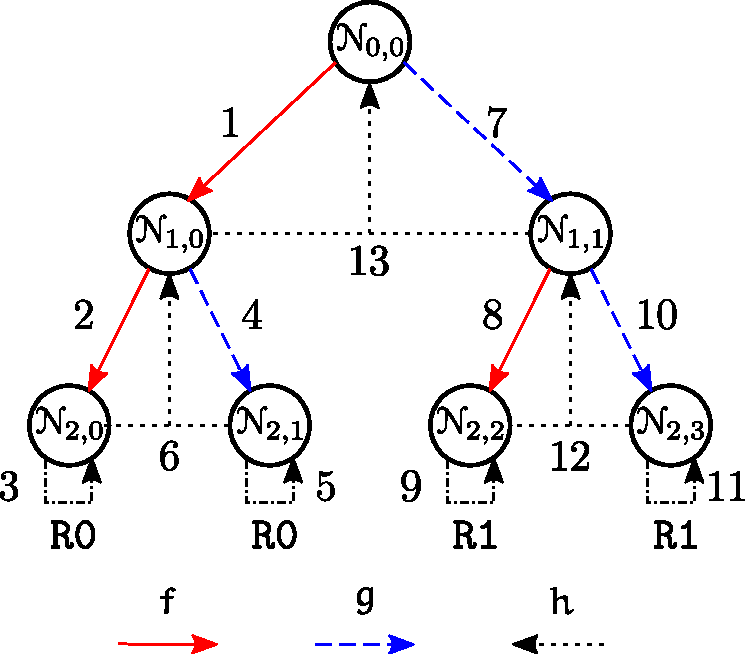
\includegraphics[width=\linewidth]{main/ch2_fig/unrolled_tree}
  \label{fig:unrolled_tree}
  \end{minipage}%
  }
  \caption{Déroulage du code source décrivant l'algorithme de décodage SC non élagué d'un code polaire (4,2) systématique.}
  \label{fig:unrolling}
\end{figure}

\subsection{Cibles}

\section{Généricité et Flexibilité d'un décodeur de codes polaire}

\label{sec:gen_scl}
\subsection{Définitions}
Les implémentations logicielles proposées sont génériques et flexibles. Afin d'éviter toute ambiguïté, ces termes doivent être définis précisément.
D'une part, le terme \textit{généricité} définit la capacité d'un décodeur à supporter n'importe quel encodage.
En effet, dans le contexte de télécommunications mobiles, les paramètres de l'encodeur changent constamment pour s'adapter au canal, en utilisant des méthodes adaptatives de modulation et de codage \cite{dahlman_4g:_2013} (AMC : Adaptive Modulation and Coding). Ainsi, les tailles de mot de code, les rendements, les ensembles de bits gelés évoluent. Des patrons de poinçonnage sont souvent nécessaires et des CRC sont concaténés pour détecter les erreurs et permettre des méthodes de transmission à demande de répétition automatique (ARQ : Automatic Repeat reQuest) ou leur équivalent hybride (HARQ : Hybrid ARQ). Un décodeur générique devra donc supporter toutes les combinaison possibles de chacun de ces paramètres.

D'autre part, le terme \textit{flexibilité} s'applique aux paramétrage de l'algorithme et des méthodes d'implémentation du décodeur, indépendamment du schéma d'encodage. Ces paramétrages-ci ne sont généralement pas imposés par le standard. Dans le cas de l'algorithme SCL, les paramètres suivants sont concernés : les variantes de l'algorithme (FASCL, PASCL), le format de quantification des données (virgule flottante ou fixe, nombre de bits), la taille de la liste $L$ ou encore l'élagage de l'arbre de décodage. La flexibilité du décodeur amène des degrés de liberté permettant des compromis entre pouvoir de correction, latence et débit, pour un schéma d'encodage donné.

Comme il sera détaillé dans les sections suivantes, tous les paramètres de généricité et de flexibilité cités sont pris en compte dans les décodeurs proposés. Ils sont déterminés par des fichiers de configurations, lus au moment de l'exécution. Aucune compilation n'est nécessaire en cas de changement de n'importe quel paramètre. De ce choix découle le fait que nous n'utilisons pas la technique de déroulage présentée en Section \ref{subsec:unroll}. En effet, cette technique implique la génération d'un code source pour chaque combinaison de paramètres différente comme proposé en \cite{sarkis_autogenerating_2014} pour l'algorithme SC.

\subsection{Généricité}

\begin{figure}[t]
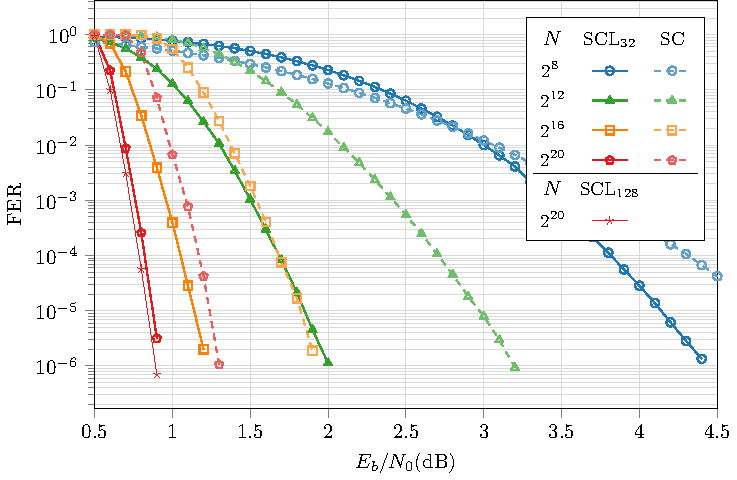
\includegraphics[width=\textwidth]{main/ch2_fig/curves/code/tikz/code}
\caption{Performances de décodage des algorithme SC et CASCL pour des tailles importantes de mots de code, $R=1/2$, CRC $c=32$ (GZip)}
\label{fig:large_scl}
\end{figure}

Les implémentations de décodeurs proposées gèrent n'importe quelle taille de mot de code. De plus, les débits des décodeurs étant compétitifs, il est possible d'explorer d'importantes tailles de mots de code ($N\geq2^{12}$) conjointement à des profondeurs de liste importante ($L \geq 32$), comme montré dans la Figure~\ref{fig:large_scl}. $N$ prend des valeurs allant de $2^8$ à $2^{20}$ et le rendement du code est $R=1/2$. Le CRC utilisé est défini dans le standard GZip, sa longueur est $c=32$ et son polunôme \texttt{0x04C11DB7}. Des simulations pour de telle valeurs de paramètres sont rares dans la littérature, et montrent que, bien que l'algorithme SCL ait été conçu pour améliorer les performances de décodage des codes polaires pour de petites tailles ($N<2^{12}$), son utilisation pour des codes de grande taille apporte également un important gain. Dans le cas où $N=2^{12}$, l'utilisation de l'algorithme CASCL avec une taille de liste $L=32$ amène un gain de d'environ 1.2 dB lorsque le FER est égal à $10^{-5}$. Ce gain diminue cependant lorsque $N$ augmente, avec 0.75 dB pour $N=2^{16}$ et 0.5 dB pour $N=2^{20}$. Des simulations ont également été réalisées pour une profondeur de liste $L=128$. Elles montrent que le gain par rapport à $L=32$ n'est pas significatif.

\subsection{Flexibilité}
Les paramètres de flexibilité sont eux aussi configuré lors de l'exécution du programme. Ils permettent des compromis divers entre la latence, le débit et les performance de correction. Ainsi, l'algorithme de décodage peut être ajusté finement pour un code polaire donné. Dans les sections à venir, ces paramètres de flexibilité sont détaillés et leurs effets analysés.

\subsubsection{Profondeur de la liste}
\begin{figure}[t]
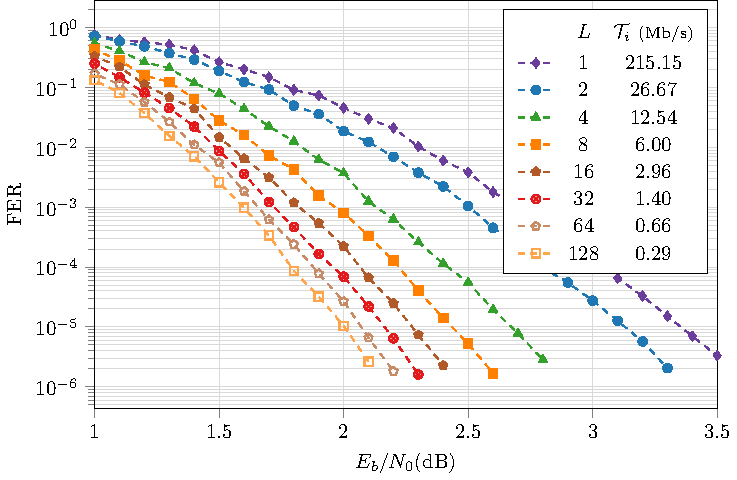
\includegraphics[width=\textwidth]{main/ch2_fig/curves/L/tikz/L}
\caption{Performances de décodage et débits de l'algorithme CASCL pour différentes valeurs de $L$ d'un code polaire ($2048,1024$) concaténé à un CRC $c=32$ (GZip).}
\label{fig:scl_l_thr}
\end{figure}
La profondeur de la liste impacte directement le pouvoir de correction et la complexité de l'algorithme. En Figure~\ref{fig:scl_l_thr} sont représentées les courbes de FER et les débits obtenus pour l'algorithme de décodage CASCL d'un code polaire ($2048$,$1024$). La complexité calculatoire augmente linéairement : le débit est approximativement doublé lorsque $L$ est doublé. Le seul cas ne respectant pas cette assomption est celui pour lequel $L=1$ qui correspond à l'algorithme SC, bien plus rapide puisque n'ayant pas à effectuer les calculs associés à l'algorithme SCL comme le tri, la génération des candidats, le calcul du CRC. Le FER évolue également avec $L$. \`A partir de $L\geq4$ et $E_b/N_0=2$, le FER est divisé par deux lorsque $L$ est doublé.

\subsubsection{Paramétrage fin de l'élagage}
L'élagage, tel que défini en Section~\ref{subsec:pruning} est paramétrable très finement dans les implémentations de décodeurs polaires proposées. Tout d'abord, chaque type de \noeud (\texttt{R0}, \texttt{R1}, \texttt{REP} et \texttt{SPC} peut être activé ou désactivé séparément. Cette capacité est utile pour explorer l'impact de l'utilisation de chaque \noeud sur le débit codé.

Il faut ici faire la distinction entre le débit codé  et le débit d'information. Soit $\mathcal{T}_F$, le nombre de trames décodées par seconde. Alors le débit d'information est $\mathcal{T}_i=K\mathcal{T}_F$, soit le nombre de bits d'informations décodés par seconde, et le débit codé est $\mathcal{T}_c=N\mathcal{T}_F$.

Pour explorer l'impact de l'utilisation des \noeuds sur le débit, il est  plus pertinent d'utiliser le débit codé. En effet, si l'on utilisait le débit d'information dans la Figure~\ref{fig:nodes}, le rendement du code biaiserait les débits : le débit des codes à haut rendement auraient un débit bien supérieurs aux codes à faibles rendement.
\begin{figure}[t]
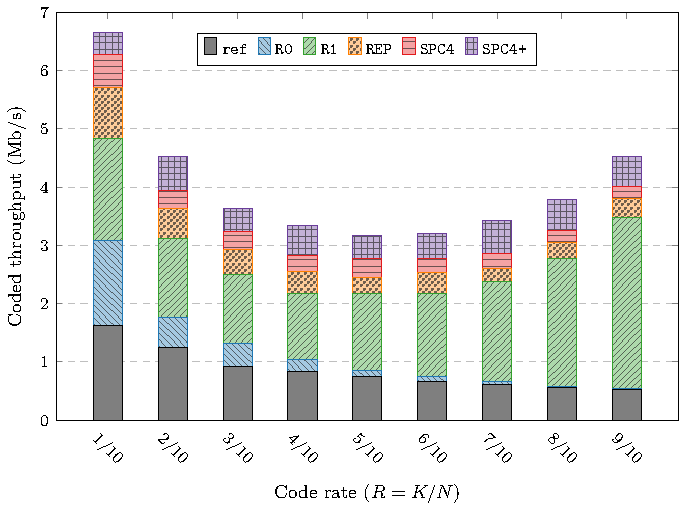
\includegraphics[width=\textwidth]{main/ch2_fig/curves/tree/tikz/tree}
\caption{Impact de l'activation des \noeuds d'élagage de l'algorithme CASCL, $N=2048$, $L=32$, $c=32$.}
\label{fig:nodes}
\end{figure}

\begin{figure}[t]
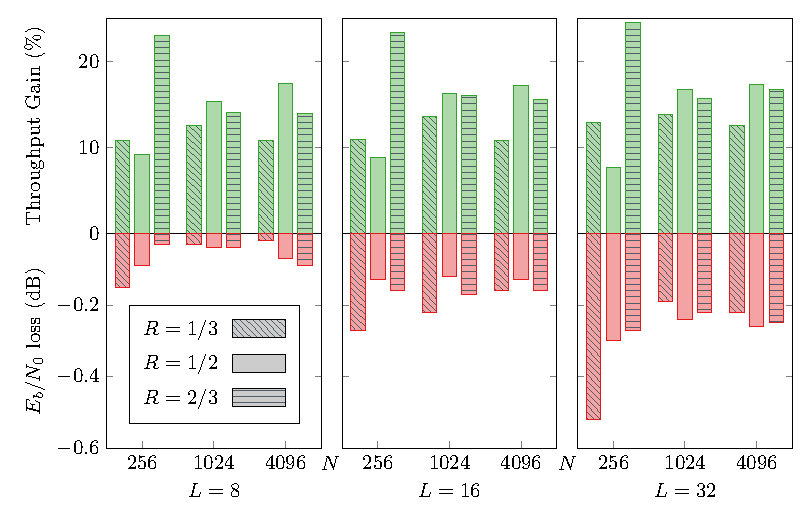
\includegraphics[width=\textwidth]{main/ch2_fig/curves/thr_spc/tikz/thr_spc_diff}
\caption{Effets de l'utilisation des \noeuds \texttt{SPC4+} dans l'algorithme CASCL à un FER de $10^{-5}$}
\label{fig:spc_impact}
\end{figure}

Le débit codé de l'algorithme non élagué (\texttt{ref}) diminue lorsque le rendement augmente. Cela s'explique par le fait que les feuilles de rendement 1, plus nombreuses dans les codes à hauts rendements, sont plus long à décoder que les feuilles de rendement 0. En effet, dans l'algorithme SCL, le traitement d'une feuille de rendement 0 correspond à la mise à jour de métriques, tandis que le traitement d'une feuille de rendement 1 correspond à la génération de candidats, la mise à jour de leurs métriques, le tri de celles-ci, et des duplications d'arbres de décodage.

Les aires hachurées en diagonales représentent l'amélioration des performances de décodage lorsque les \noeuds \texttt{R0} et \texttt{R1} de taille supérieures à un (c'est à dire les \noeuds plus haut que les feuilles) sont utilisés pour l'élagage. De manière attendue, l'élagage \texttt{R1} est plus efficace pour les codes à haut rendement et, inversement, l'élagage \texttt{R0} est plus efficace pour les codes à faible rendement. On observe la même tendance pour l'élagage des \noeuds \texttt{REP} plus efficace pour les codes de faibles rendements, qui en contiennent également beaucoup. La tendance est moins claire pour les \noeuds \texttt{SPC}.

Il fut également observé dans \cite{sarkis_fast_2014} que lorsque la taille des \noeuds \texttt{SPC} n'est pas limitée à 4, les performances de décodage peuvent être dégradées. Dans les implémentations proposées, le choix a été fait de donner la possibilité de paramétrer finement la taille des \noeuds activés pour chaque type de \noeuds. En conséquence, leur taille est limitée à 4 dans les aires labellisées \texttt{SPC4} dans la figure \ref{fig:nodes}. Les \noeuds \texttt{SPC4+} sont de tailles supérieures. 

Selon nos expérimentations, la dégradation des performances de correction due à l'utilisation des \noeuds \texttt{SPC4+} n'est pas systématique mais dépendante des caractéristique du code polaire considéré. La Figure~\ref{fig:spc_impact} montre dans sa partie supérieure que les gains en débit sont significatifs selon nos expérimentations. Ils sont compris entre 8\% et 20\% selon les cas, c'est-à-dire selon la profondeur de la liste, la taille du mot de code et le rendement. La partie inférieure de la figure montre pour sa part la dégradation des performances de décodage. Pour une profondeur de liste $L=8$, en dehors d'une configuration particulière ($N=256$, $R=1/3$), la dégradation du SNR pour un FER de $10^{-5}$ est inférieure à 0.1 dB. Tandis une taille de liste $L=32$ la dégradation est généralement légèrement supérieure à 0.2 dB. Encore une fois le cas ($N=256$, $R=1/3$) est désavantageux, avec une dégradation d'environ 0.5 dB.

En conclusion, l'élagage de l'arbre permet des améliorations significatives du débit des implémentations logicielle de l'algorithme SCL. Toutefois le traitement des \noeuds \texttt{SPC4+} décrit dans \cite{sarkis_fast_2016} peut provoquer une dégradation des performances de décodage dont l'importance dépend des paramètres de l'algorithme. Des tests doivent donc être réalisés pour connaître leur impact. Or la flexibilité de conception des implémentations proposées permettent de réaliser facilement de tels tests, grâce à la possibilité d'activer dynamiquement l'utilisation de n'importe quel type de \noeud spécialisé de n'importe quelle taille.

\subsubsection{Quantification}

\begin{figure}
\centering
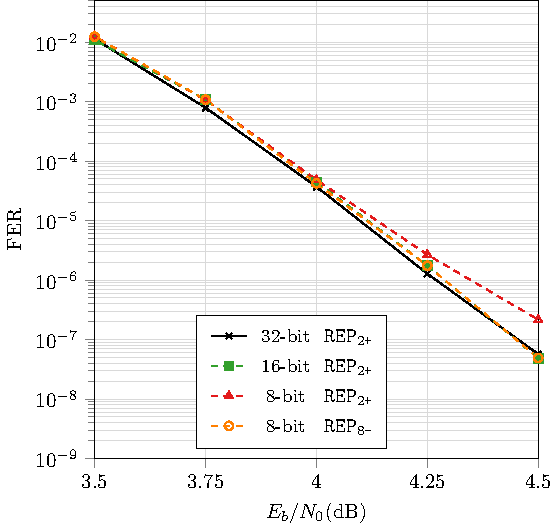
\includegraphics{main/ch2_fig/curves/bfer/tikz/bfer_rep}
\caption{Impact de l'utilisation des \noeuds de répétition sur des implémentations quantifiées.}
\label{fig:bfer_rep}
\end{figure}

La quantification des variables internes de l'algorithme de décodage sont un important paramètre du décodeur. En effet les sommes partielles et les LLRs peuvent être représentées en virgule fixe sur un nombre réduits de bits \cite{balatsoukas-stimming_llr-based_2015}. Si des implémentations logicielles quantifiées de l'algorithme SC ont déjà été proposées \cite{giard_low-latency_2016}, les décodeurs proposés constituent, à la connaissance de l'auteur, la première implémentation logicielle de l'algorithme SCL permettant de représenter les LLRs et les métriques de chemin sur 8 ou 16 bits. Ces représentations permettent d'augmenter le parallélisme grâce à l'utilisation des instructions SIMD. Pour que ces quantifications fonctionnent, des précautions doivent être prises. Tout d'abord, pour les représentations 8 bits, les LLRs et les métriques sont saturées entre -127 et +127 après chaque opération. De plus les métriques de chemin sont normalisées après chaque opération de duplication et sélection de candidats : la valeur la plus faible des métriques de chemin est soustraite à chacune d'entre elles. La Figure~\ref{fig:rep_impact} montre les performances de l'algorithme CASCL pour différentes représentations des LLRs : 8 bits, 16 bits à virgule fixe et 32 bits à virgule flottante. Si les courbes 32 bits et 16 bits sont confondues et montrent que la représentation sur 16 bits ne dégrade pas les performances, il est possible d'observer que des dégradations apparaissent pour la courbe 8 bits, labellisée \texttt{REP2+}. Après étude, il s'avère que ces dégradations sont dues au traitement des \noeuds de répétition. En effet, lors de ce traitement, comme détaillé en Section \ref{subsec:pruning}, il faut ajouter tous les LLR du \noeud considéré. Or pour un \noeud de répétition de grande taille, cette addition sur 8 bits peut causer un débordement. On peut voir que lorsque les \noeuds de répétition de taille supérieure à 8 sont désactivés (\texttt{REP8-}), ces débordements n'ont plus lieu et les performances deviennent quasiment identiques à celles correspondant à la représentation 32 bits en virgule flottante.

Dans le tableau \ref{tab:quantif} sont listés la latence \og pire cas \fg ($\mathcal{L}_{PC}$), la latence moyenne ($\mathcal{L}_moy$) et le débit d'information ($\mathcal{T}_i$) des algorithmes adaptatifs, PASCL et FASCL, pour les différentes quantifications. Dans le cas de la quantification 8 bits les \noeuds répétitions de taille supérieure à 8 sont désactivés afin d'effectuer les mesures à performances de décodage égales. Les représentations à virgule fixe réduisent dans la majorité des cas la latence moyenne, surtout dans les régions à haut SNR. Ceci est dû au fait que le gain dû à la quantification est plus important pour l'algorithme SC que pour l'algorithme SCL. Or, dans le cas des algorithmes adaptatifs, plus le SNR est grand, plus il est probable que le décodage SC suffise et qu'il n'y ait pas besoin de réaliser les décodages SCL. Ainsi, un débit de 425.9 Mb/s est atteint en représentation sur 8 bits pour l'algorithme FASCL, soit une augmentation de 80 Mb/s en comparaison avec la représentation sur 32 bits.
\begin{figure}[t]
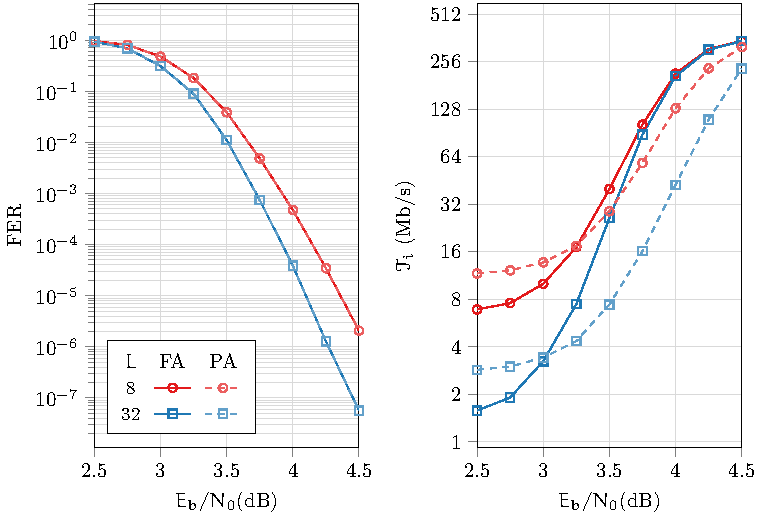
\includegraphics{main/ch2_fig/curves/ascl/tikz/ascl}
\caption{Performances de décodage et débits des algorithmes de décodage PASCL et FASCL pour un code polaire ($2048$,$1723$), $L=32$, et CRC $c=32$ GZip.}
\label{fig:ascl_perfs}
\end{figure}[t]

  \begin{table}[t]
    \renewcommand{\arraystretch}{1.1}
    \centering
    \caption{Comparaison de débits et latences des algotihmes SCL adaptatifs pour des représentations en virgule flottante (32 bits) et virgule fixe (16 et 8 bits). Code polaire ($2048$,$1723$), $L=32$, CRC $c=32$ (GZip)}
    \label{tab:quantif}
    {\small\resizebox{\linewidth}{!}{
    \begin{tabular}{r | c | c || c | c || c | c || c | c}
      \multirow{2}{*}{\textbf{Décodeur}} & \multirow{2}{*}{\textbf{Quantif.}} & \multirow{2}{*}{$\bm{\mathcal{L}_{PC}}$} & \multicolumn{2}{c ||}{\textbf{3.5 dB}} & \multicolumn{2}{c ||}{\textbf{4.0 dB}} & \multicolumn{2}{c}{\textbf{4.5 dB}} \\
      \cline{4-9}
      & & & $\bm{\mathcal{L}_{moy}}$ & $\bm{\mathcal{T}_i}$ & $\bm{\mathcal{L}_{moy}}$ & $\bm{\mathcal{T}_i}$ & $\bm{\mathcal{L}_{moy}}$ & $\bm{\mathcal{T}_i}$ \\
      % \hline
      \hline
      \multirow{3}{*}{PA-SSCL} & 32-bit &  635 & 232.3 &   7.6 & 41.7 &  42.1 & 7.4 & 237.6 \\
      %\cline{3-9}
                               & 16-bit &  622 & 219.6 &   8.0 & 40.1 &  43.8 & 6.6 & 267.5 \\
      %\cline{3-9}
                               &  8-bit &  651 & 232.4 &   7.6 & 41.2 &  42.6 & 6.5 & 268.3 \\
      \hline
      \multirow{3}{*}{FA-SSCL} & 32-bit & 1201 &  67.2 &  26.1 &  8.5 & 207.8 & 5.1 & 345.5 \\
      %\cline{3-9}
                               & 16-bit & 1198 &  68.7 &  25.6 &  7.7 & 225.7 & 4.3 & 408.7 \\
      %\cline{3-9}
                               &  8-bit & 1259 &  71.8 &  24.4 &  7.7 & 227.3 & 4.1 & 425.9 \\
    \end{tabular}
    }}
  \end{table}

\subsubsection{Support de différentes variantes algorithmiques}
Les deux versions adaptatives de l'algorithme SCL que sont les algorithmes partiellement et complètement adaptatifs (PASCL et FASCL) présentent des débits différents suivant le rapport signal à bruit $E_b/N_0$ considéré, comme montré en Figure~\ref{fig:ascl_perfs}. Pour de faibles valeurs de SNR, l'algorithme PASCL et plus avantageux, mais pour des valeurs plus élevées c'est l'algorithme FASCL qui prend l'avantage. Cependant, dans tous les cas et comme décrit en Section \ref{subsubsec:adaptive}, la latence \og pire cas \fg, autrement dit le temps nécessaire maximum que peut prendre le décodage d'une trame, est plus élevée dans le cas de l'algorithme FASCL. Ce fait est vérifié par la mesure comme reporté dans le Tableau~\ref{tab:quantif}.

Voici donc présentés les caractères génériques et flexibles des décodeurs proposés. Cependant, l'objectif de ces implémentations est également d'être compétitives avec les décodeurs de la littérature du point de vue du débit et de la latence. Des améliorations permettant cette compétitivité sont présentées dans la section suivante.

\section{Optimisations de l'implémentation logicielle des décodeurs liste}
\label{sec:opti_scl}
Trois contributions originales sont présentées dans cette section. la première porte sur l'utilisation nouvelle d'un algorithme de tri des métriques et des LLRs, la seconde sur l'accélération du contrôle de redondance cyclique et la troisième concerne la gestion des sommes partielles. 

\subsection{Algorithme de tri}
Des algorithmes de tri sont nécessaires lors de plusieurs étapes durant l'algorithme SCL. Les métriques de chemins sont triées pour sélectionner les candidats lors des étapes de duplication (étapes (i+1) et (i+3) de la Figure~\ref{fig:scl}). De plus les LLRs doivent être triés lors du traitement des \noeuds \texttt{R1} et \texttt{SPC}. \`A cause d'un manque de détails dans la description de l'implémentation du tri dans \cite{sarkis_fast_2016}, sa reproduction est difficile. Différentes méthodes de tri sont donc explorées.

Tout d'abord, lors du traitement des \noeuds \texttt{R1}, il est nécessaire d'identifier les deux LLRs les moins fiables, c'est à dire ceux possédant la valeur absolue la plus faible. Or, la méthode optimale, du point de vue du nombre de comparaisons, d'identifier les deux plus petits (ou les deux plus grands) éléments d'un ensemble est présentée dans \cite{schreier_tournament_1932} et reportée dans \cite{knuth_art_1973}. Cette méthode sera par la suite dénommée méthode de Schreier du nom de son auteur. Elle se réalise en deux étapes, présentées en Figure~\ref{fig:schreier_sort}. La première étape est l'identification du plus petit élément par la traversée d'un arbre binaire. Ensuite, cet élément est éliminé, et la branche sur laquelle il se trouvait est rejouée. Le deuxième élément le plus petit est ainsi identifié.

Cette méthode s'est avérée être la plus rapide expérimentalement de toutes celles qui ont été testées : \textit{Batcher's merge exchange}, tri par bulle, tri \textit{quick-sort}, tri par tas implémenté dans la librairie standard. Elle l'était également dans les cas testés pour les \noeuds de type \texttt{SPC}. Une étude comparée montre que la méthode de Schreier est également pertinente pour le tri des métriques, puisqu'il s'agit de faire un tri partiel d'une liste de métriques.

\begin{figure}
\centering
\subfloat[Identification du plus petit élément.]{
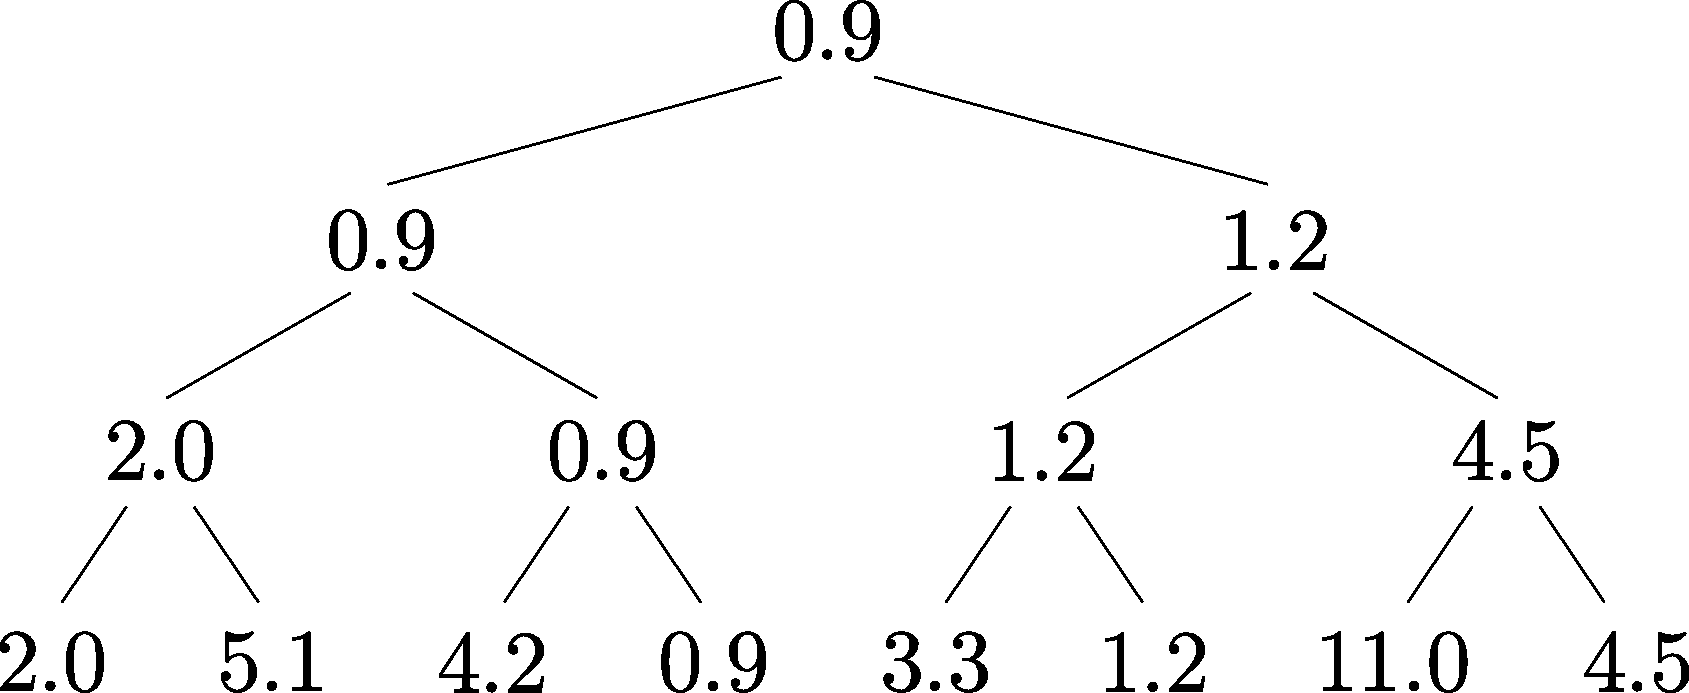
\includegraphics[width=0.75\textwidth]{main/ch2_fig/sorting_a}
\label{fig:sorting_a}
}
\\
\subfloat[Identification du deuxième plus petit élément.]{
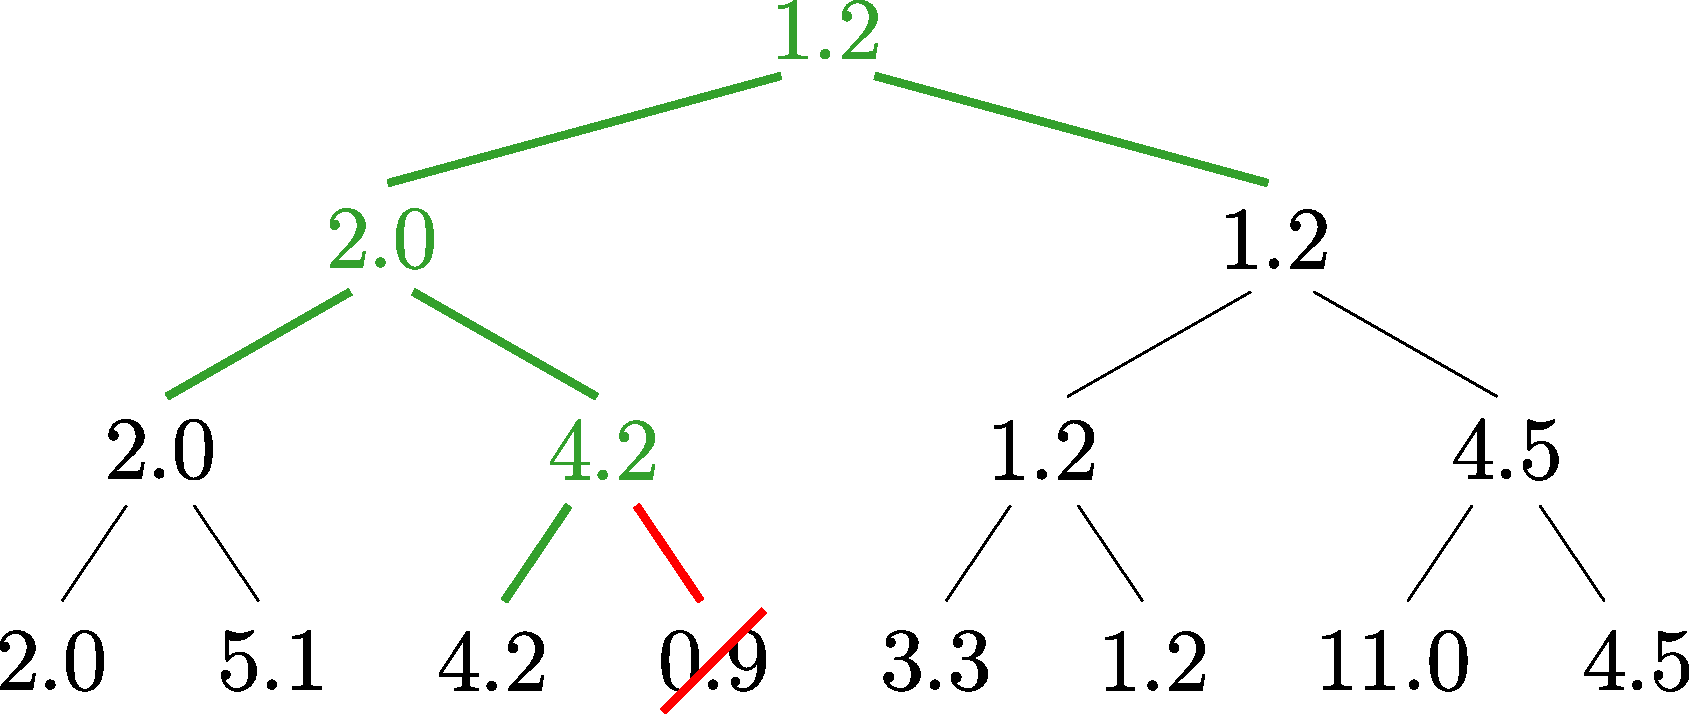
\includegraphics[width=0.75\textwidth]{main/ch2_fig/sorting_b}
\label{fig:sorting_b}
}
\caption{Méthode de Schreier}
\label{fig:schreier_sort}
\end{figure}

\subsection{Accélération du contrôle de redondance cyclique}
Par profilage de l'exécution d'un décodeur SCL adaptatif, il est possible d'observer que beaucoup de temps est passé à réaliser des vérifications de CRC. En effet, la complexité calculatoire du CRC est en $O(N)$ tandis que celle du reste de l'algorithme SCL est en $O(N\log N)$. Pour les valeurs de N considérées, le premier n'est pas négligeable par rapport au second. Des méthodes d'implémentation efficaces doivent donc être utilisées. Tout d'abord, les bits sont empaquetés pour être traités 32 par 32. Les sommes partielles sont stockées au départ chacune sur un entier. Pour vérifier le CRC, 32 sommes partielles sont lues et sont stockées dans un seul entier de 32 bits. Une table de conversion est utilisée pour stocker des séquences pré calculées du CRC. La lecture de ces séquences permet de réduire la complexité calculatoire totale.

Dans les algorithmes adaptatifs, après un premier décodage de la trame par l'algorithme SC, un premier mot de code candidat de $N$ bits est proposé. Or le CRC est calculé sur les seuls $K$ bits d'information parmi les $N$ bits du mot de code. il est donc nécessaire de réaliser l'extraction des bits d'information. Le profilage des décodeurs montre que cette opération d'extraction représente une portion non négligeable du temps total de traitement du CRC. Or il est possible d'accélérer cette extraction en utilisant la connaissance que nous avons de l'emplacement des bits gelés par la connaissance des \noeuds d'élagage. En effet, la présence d'un \noeud de type \texttt{R1} de taille $M$ correspond à la présence de $M$ bits d'information consécutifs. Il est alors possible d'utiliser les unités matérielles SIMD afin de réaliser une extraction parallèle de multiples bits simultanément.


\subsection{Gestion des sommes partielles}
Dans cette section est décrite la gestion des sommes partielles dans les décodeurs proposés.
Les sommes partielles sont des décisions dures et leurs valeurs sont donc binaires. Cependant, dans les implémentations logicielles proposées, afin d'utiliser efficacement les instructions SIMD, les LLRs et les sommes partielles sont représentés sur par des entiers de même dimension, notée $Q$, en octets. Selon la représentation choisie, 32, 16 ou 8 bits, $Q$ peut donc prendre les valeurs 4, 2 ou 1. 
Dans les précédentes implémentations logicielles de l'algorithme SCL \cite{sarkis_fast_2016,sarkis_increasing_2014,shen_low-latency_2016}, un emplacement mémoire de $Q$ bits est alloué à chaque niveau de l'arbre de décodage comme décrit dans \cite{tal_list_2011}. La taille de l'emplacement mémoire associé à un niveau de l'arbre est égal à la taille des \noeuds du niveau en question. Soit $n=\log_2(N)$, le nombre total de niveaux est $n+1$ et la taille d'un \noeud au niveau $l$ est égal à $2^{n-l}$. L'empreinte mémoire pour les sommes partielles d'un arbre de décodage est égale à : 
\begin{equation}
\sum^n_{l=0}2^{n-l}=2N-1
\end{equation}
Pour l'algorithme SCL dans lequel L arbres de décodage sont nécessaires, l'empreinte mémoire totale pour l'algorithme SCL est donc $L(2N-1)$. Cependant cette empreinte mémoire peut être réduite. En effet, dans l'algorithme SC, les sommes partielles d'un \noeud donné de l'arbre de décodage ne sont utilisées qu'une fois au cours du décodage, donc ces emplacements mémoire peuvent être recyclés. Ainsi l'empreinte mémoire peut être réduite de $2N-1$ à $N$ dans l'algorithme SC \cite{leroux_hardware_2011}. De la même manière, il est possible de réduire cette empreinte mémoire de $L(2N-1)$ à $LN$ pour l'algorithme SCL.

Lors des étapes de duplication et de sélection de l'algorithme SCL, étapes $(i+1)$ et $(i+3)$ de la Figure \ref{fig:scl}, il est nécessaire de assigner les sommes partielles d'un arbre de décodage original à un nouvel arbre. Deux méthodes sont possibles pour réaliser cette assignation. La première, notée $SCL_{cpy}$, consiste à systématiquement copier les $N$ sommes partielles sauvegardée dans l'emplacement mémoire du premier arbre de décodage vers l'emplacement mémoire du second. La deuxième, présentée dans \cite{tal_list_2011}, est de réaliser cette assignation par l'utilisation de pointeurs. Ainsi, tant que les sommes partielles de chaque arbre ne diffèrent pas, ils utilisent le même emplacement mémoire. Cette méthode est notée $SCL_{ptr}$.

La méthode $SCL_{ptr}$ semble plus efficace puisqu'elle évite des copies inutiles. Cependant, nos expérimentations montrent que le surplus de calculs nécessaire à la gestion des pointeurs pénalise cette méthode pour des codes de petite et moyenne taille, comme montré en Figure~\ref{fig:scl_mem} qui représente les débits des implémentations de l'algorithme SCL utilisant chacune des méthodes, pour différentes valeurs de $N$, un rendement constant, $R=1/2$ et une profondeur de liste $L=32$. Ces courbes montrent que la méthode $SCL_{cpy}$ permet des débits plus rapides pour $N<8192$ tandis que le méthode $SCL_{ptr}$ est plus avantageuse pour des débits supérieurs. La Figure~\ref{fig:scl_mem} montre également l'impact du format utilisé pour la représentation des LLRs et des sommes partielles. Pour de très grandes valeurs de $N$, la représentation sur 8 bits est plus efficace, puisqu'elle occupe moins d'espace mémoire et que les échecs d'accès à la mémoire cache sont plus rares. 

\begin{figure}
\centering
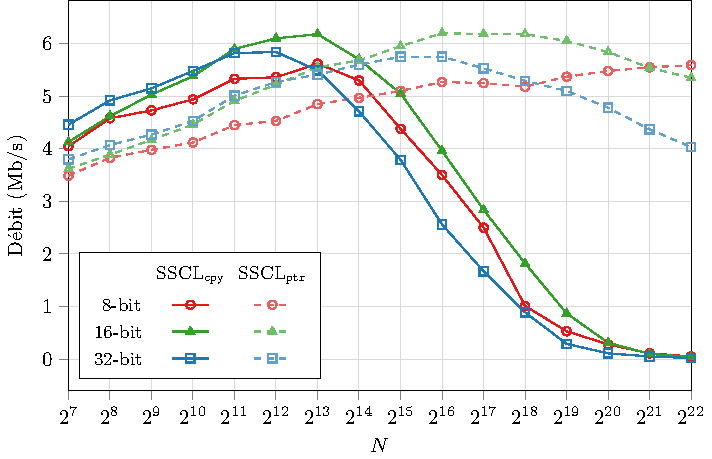
\includegraphics{main/ch2_fig/curves/thr/tikz/thr}
\caption{Comparaison des débits associés aux méthodes $SCL_{cpy}$ et $SCL_{ptr}$ pour différentes valeurs de $N$.}
\label{fig:scl_mem}
\end{figure}




\section{Mesures et comparaisons}
\label{sec:exp_scl}

Les débits et latences des implémentations proposées sont détaillées dans cette section. Tous les résultats proposés ont été générés grâce à l'outil AFF3CT \cite{aff3ct_aff3ct:_2016}. Le code source de ce logiciel est ouvert et disponible en ligne. Ainsi, tous les résultats sont facilement reproductibles. La cible matérielle est un CPU Intel i5-6600K d'architecture Skylake. Le jeu d'instruction SIMD AVX2 est utilisé. Sa fréquence pour les résultats reportés est 3.9 GHz. La compilation a été effectuée sur un OS Linux avec le compilateur C++ de GNU (version 5.4.0) et les options de compilation suivantes : \texttt{-Ofast -march=native -funroll-loops}.

\subsection{Algorithme complètement adaptatif}
L'algorithme FASCL permet d'atteindre les débits les plus élevés. Comme il est montré dans le Tableau~\ref{tab:quantif}, l'implémentation de cet algorithme avec un représentation sur 8 bits des LLRs et des sommes partielles permet d'atteindre un débit de 425 Mb/s pour un code polaire (2048,1723) et le CRC GZip de taille 32 bits lorsque $E_b/N_0=4.5dB$. Ce débit est pratiquement deux fois supérieur à celui obtenu avec l'algorithme PASCL. Le rapport signal à bruit pour lequel la différence entre PASCL et FASCL est la plus grande (380\%), est dans le domaine où le FER est compris entre $10^{-3}$ et $10^{-5}$. Il s'agit du domaine ciblé pour les communications sans fils comme LTE ou le futur réseau 5G. Dans ces conditions, le débit de l'algorithme FASCL est d'approximativement 230Mb/s tandis que celui de PASCL est d'approximativement 40 Mb/s. Rappelons toutefois que la latence dans le pire cas est plus élevée dans le cas de l'algorithme FASCL.

    \begin{table}[t]
      \centering
      \caption{Comparaison des débits et latences des décodeurs proposés avec des décodeurs de l'état de l'art. Représentation des LLRs et sommes partielles sur 32 bits. Code polaire (2048,1723), $L=32$, CRC GZip $c=32$.}
      \label{tab:res}
      {\small\resizebox{\linewidth}{!}{
      \begin{tabular}{r|r|c|c c c}
        \multirow{2}{*}{\textbf{Target}} & \multirow{2}{*}{\textbf{Décodeur}}  & \multirow{1}{*}{\textbf{$\bm{\mathcal{L}_{PC}}$}} & \multicolumn{3}{c}{$\bm{\mathcal{T}_i}$ (Mb/s)} \\
        \cline{4-6}
        &                           & ($\mu s$)                          & \textbf{3.5 dB} & \textbf{4.0 dB} & \textbf{4.5 dB} \\
        \hline
        % \hline
        \multirow{1}{*}{i7-4790K}
        & CASCL \cite{shen_low-latency_2016} & 1572                           & 1.10            & 1.10            & 1.10            \\
        \hline
        \multirow{3}{*}{i7-2600}
        & CASCL \cite{sarkis_increasing_2014} & 23000                          & 0.07            & 0.07            & 0.07            \\
        & CASSCL\cite{sarkis_increasing_2014} & 3300                           & 0.52            & 0.52            & 0.52            \\
        & PASSCL \cite{sarkis_increasing_2014} & $\approx$ 3300                 & 0.9             & 4.90            & 54.0            \\
        \hline
        \multirow{3}{*}{i7-2600}
        & CASCL  \cite{sarkis_fast_2016}   & 2294                           & 0.76            & 0.76            & 0.76            \\
        & CASSCL \cite{sarkis_fast_2016}   & 433                            & 4.0             & 4.0             & 4.0             \\
        & PASSCL \cite{sarkis_fast_2016}   & $\approx$ 433                  & 8.6             & 33.0            & 196.0           \\
        \hline
        \multirow{4}{*}{i7-2600}
        & CASCL proposé                    & 4819                           & 0.37            & 0.37            & 0.37            \\
        & CASSCL proposé                   & 770                            & 2.3             & 2.3             & 2.3             \\
        & PASSCL proposé                   & 847                            & 5.5             & 31.1            & 168.4           \\
        & FASSCL proposé                   & 1602                           & 19.4            & 149.0           & 244.3           \\
        \hline
        \multirow{4}{*}{i5-6600K}
        & CASCL proposé                    & 3635                           & 0.48            & 0.48            & 0.48            \\
        & CASSCL proposé                   & 577                            & 3.0             & 3.0             & 3.0             \\
        & PASSCL proposé                   & 635                            & 7.6             & 42.1            & 237.6           \\
        & FASSCL proposé                   & 1201                           & 26.1            & 207.8           & 345.5           \\
      \end{tabular}
      }}
    \end{table}

\subsection{Comparaison avec l'état de l'art}
Les débits et latences des décodeurs proposés sont listés et comparés avec ceux de certains décodeurs de l'état de l'art dans le tableau \ref{tab:res}. Pour tous les décodeurs, les \noeuds SPC4+ ne sont pas utilisés afin de ne pas dégrader les performances de décodage. La latence donnée dans le Tableau \ref{tab:res} est la latence \og pire cas \fg et le débit est le débit d'information moyen. La première version, CASCL, est l'implémentation de l'algorithme CASCL sans aucun élagage tandis que les versions notées CASSCL, FASSCL et PASSCL utilisent l'élagage de l'arbre. Le débit du décodeur CASSCL proposé (2.3 Mb/s) est seulement divisé par deux lorsque l'on compare avec l'implémentation spécifique déroulée de l'algorithme CASSCL décrite en \cite{sarkis_fast_2016} (4.0 Mb/s). Elle est approximativement 4 fois plus rapide que l'implémentation générique proposée en \cite{sarkis_increasing_2014} (0.52 Mb/s) et 2 fois plus rapide que celle proposée en \cite{shen_low-latency_2016}, ceci grâce aux améliorations algorithmiques proposées en Section \ref{sec:opti_scl}. De plus, les implémentations proposées présentent une flexibilité et une généricité bien plus grandes que celles proposées dans \cite{sarkis_increasing_2014,shen_low-latency_2016}. En effet, les représentations quantifiées, la possibilité de définir des patrons de poinçonnage et la possibilité d'utiliser les algorithmes adaptatifs n'étaient pas données. En utilisant la même cible matérielle (i7-2600), l'implémentation de l'algorithme PASSCL présente des débits proches de l'implémentation spécifique déroulée de \cite{sarkis_fast_2016}, tandis que le débit obtenu pour l'algorithme FASSCL est lui bien meilleur (jusqu'à 244 Mb/s pour $E_b/N_0=4.5dB$).


\section{Conclusion}
